\documentclass[aspectratio=169]{../latex_main/tntbeamer}  % you can pass all options of the beamer class, e.g., 'handout' or 'aspectratio=43'
\usepackage{dsfont}
\usepackage{bm}
\usepackage[english]{babel}
\usepackage[T1]{fontenc}
%\usepackage[utf8]{inputenc}
\usepackage{graphicx}
\graphicspath{ {./figures/} }
\usepackage{algorithm}
\usepackage[ruled,vlined,algo2e,linesnumbered]{algorithm2e}
\usepackage{hyperref}
\usepackage{booktabs}
\usepackage{mathtools}

\usepackage{amsmath,amssymb}

\DeclareMathOperator*{\argmax}{arg\,max}
\DeclareMathOperator*{\argmin}{arg\,min}

\usepackage{amsbsy}
\newcommand{\vect}[1]{\bm{#1}}
%\newcommand{\vect}[1]{\boldsymbol{#1}}

\usepackage{pgfplots}
\pgfplotsset{compat=1.16}
\usepackage{tikz}
\usetikzlibrary{trees} 
\usetikzlibrary{shapes.geometric}
\usetikzlibrary{positioning,shapes,shadows,arrows,calc,mindmap}
\usetikzlibrary{positioning,fadings,through}
\usetikzlibrary{decorations.pathreplacing}
\usetikzlibrary{intersections}
\pgfdeclarelayer{background}
\pgfdeclarelayer{foreground}
\pgfsetlayers{background,main,foreground}
\tikzstyle{activity}=[rectangle, draw=black, rounded corners, text centered, text width=8em]
\tikzstyle{data}=[rectangle, draw=black, text centered, text width=8em]
\tikzstyle{myarrow}=[->, thick, draw=black]

% Define the layers to draw the diagram
\pgfdeclarelayer{background}
\pgfdeclarelayer{foreground}
\pgfsetlayers{background,main,foreground}

% Requires XeLaTeX or LuaLaTeX
%\usepackage{unicode-math}

\usepackage{fontspec}
%\setsansfont{Arial}
\setsansfont{RotisSansSerifStd}[ 
Path=../latex_main/fonts/,
Extension = .otf,
UprightFont = *-Regular,  % or *-Light
BoldFont = *-ExtraBold,  % or *-Bold
ItalicFont = *-Italic
]
\setmonofont{Cascadia Mono}[
Scale=0.8
]

% scale factor adapted; mathrm font added (Benjamin Spitschan @TNT, 2021-06-01)
%\setmathfont[Scale=1.05]{Libertinus Math}
%\setmathrm[Scale=1.05]{Libertinus Math}

% other available math fonts are (not exhaustive)
% Latin Modern Math
% XITS Math
% Libertinus Math
% Asana Math
% Fira Math
% TeX Gyre Pagella Math
% TeX Gyre Bonum Math
% TeX Gyre Schola Math
% TeX Gyre Termes Math

% Literature References
\newcommand{\lit}[2]{\href{#2}{\footnotesize\color{black!60}[#1]}}

%%% Beamer Customization
%----------------------------------------------------------------------
% (Don't) Show sections in frame header. Options: 'sections', 'sections light', empty
\setbeamertemplate{headline}{empty}

% Add header logo for normal frames
\setheaderimage{
	% 
\includegraphics[height=\logoheight]{figures/TNT_darkv4.pdf}
	
\includegraphics[height=\logoheight]{../latex_main/figures/luh_logo_rgb_0_80_155.pdf}
	% 
\includegraphics[height=\logoheight]{figures/logo_tntluh.pdf}
}

% Header logo for title page
\settitleheaderimage{
	% 
\includegraphics[height=\logoheight]{figures/TNT_darkv4.pdf}
	
\includegraphics[height=\logoheight]{../latex_main/figures/luh_logo_rgb_0_80_155.pdf}
	% 
\includegraphics[height=\logoheight]{figures/logo_tntluh.pdf}
}

% Title page: tntdefault 
\setbeamertemplate{title page}[tntdefault]  % or luhstyle
% Add optional title image here
%\addtitlepageimagedefault{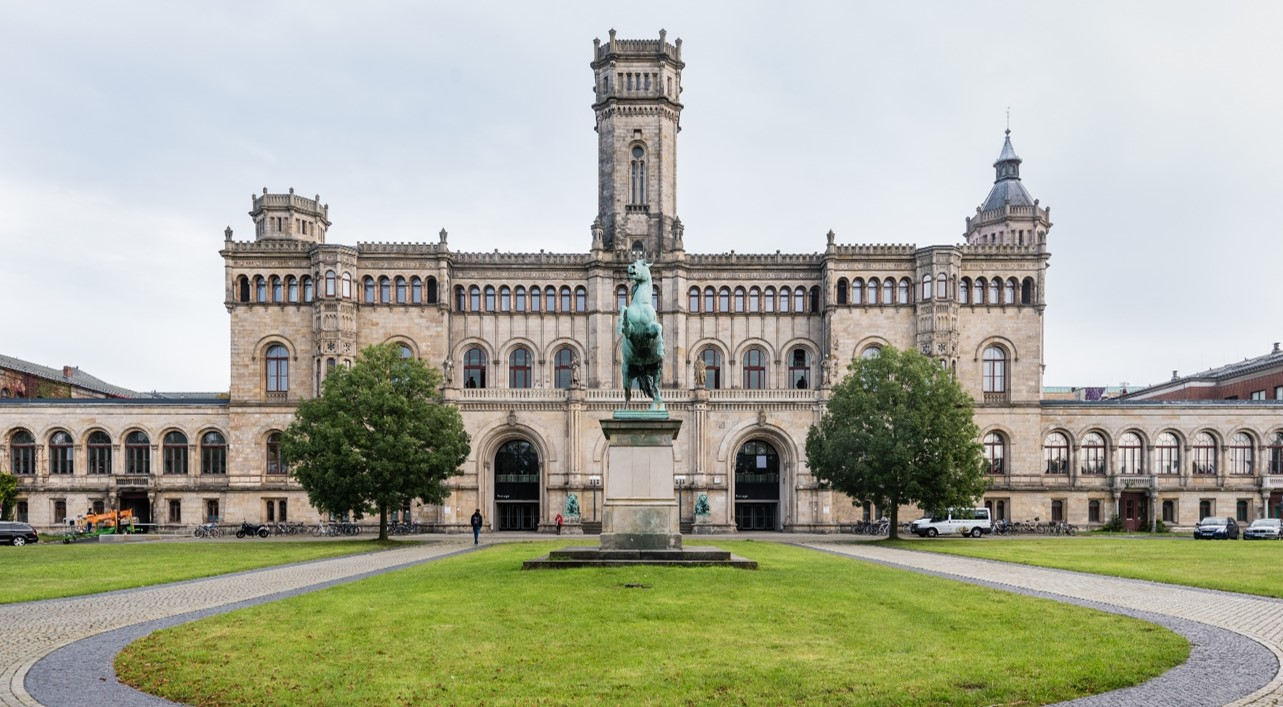
\includegraphics[width=0.65\textwidth]{figures/luh_default_presentation_title_image.jpg}}

% Title page: luhstyle
% \setbeamertemplate{title page}[luhstyle]
% % Add optional title image here
% \addtitlepageimage{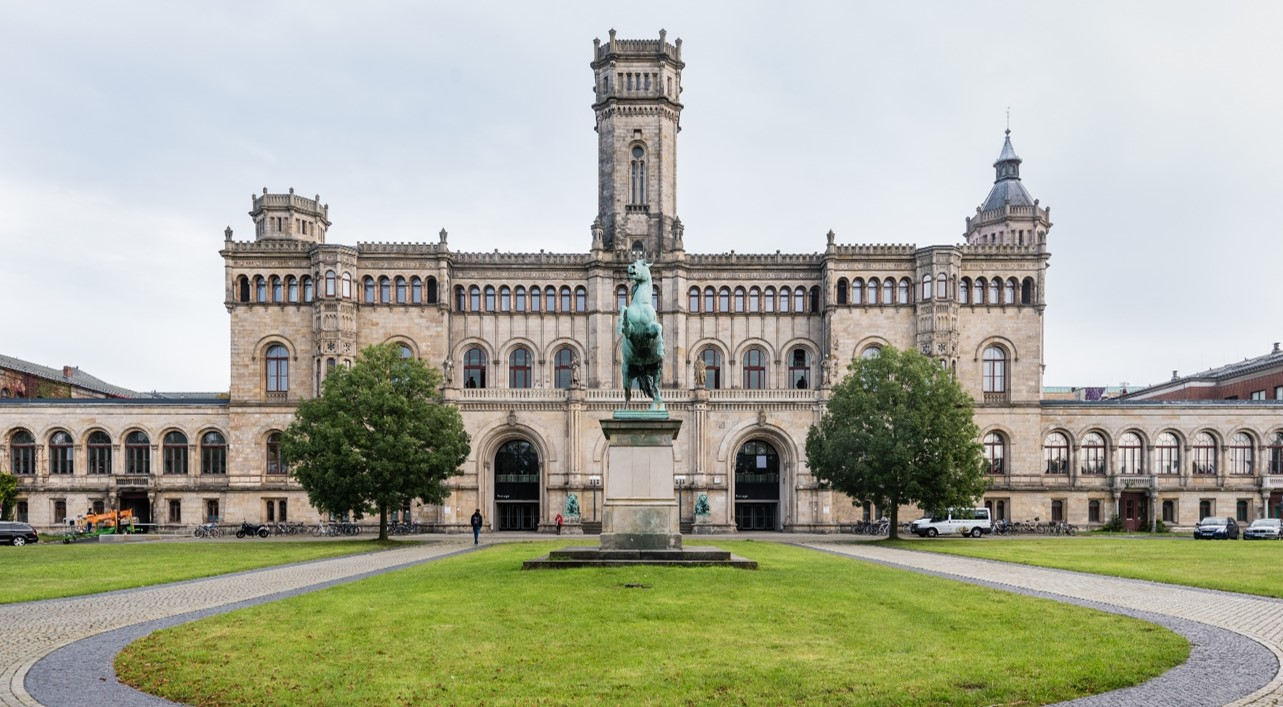
\includegraphics[width=0.75\textwidth]{figures/luh_default_presentation_title_image.jpg}}

\author[Abedjan \& Lindauer]{Ziawasch Abedjan \& Marius Lindauer\\[1em]
	
\includegraphics[height=\logoheight]{../latex_main/figures/luh_logo_rgb_0_80_155.pdf}\qquad
	
\includegraphics[height=\logoheight]{../latex_main/figures/DBIS_Kurzlogo.png}\qquad

\includegraphics[height=\logoheight]{../latex_main/figures/TNT_darkv4}\qquad

\includegraphics[height=\logoheight]{../latex_main/figures/L3S.jpg}	}
\date{Summer Term 2022; \hspace{0.5em} {
\includegraphics[height=1.5em]{../latex_main/figures/Cc-by-nc-sa_icon.svg.png}}; based on \href{https://ds100.org/fa21/}{[DS100]}
}


%%% Custom Packages
%----------------------------------------------------------------------
% Create dummy content
\usepackage{blindtext}

% Adds a frame with the current page layout. Just call \layout inside of a frame.
\usepackage{layout}


%%% Macros
%\renewcommand{\vec}[1]{\mathbf{#1}}
% \usepackage{bm}
%\let\vecb\bm

\title[Visualization]{DS: Visualization}
\subtitle{Transformations}

\graphicspath{ {./figure/} }
%\institute{}


\begin{document}
	
	\maketitle
	\begin{frame}{Transforming data can reveal patterns}
	    \begin{figure}
	        \centering
	        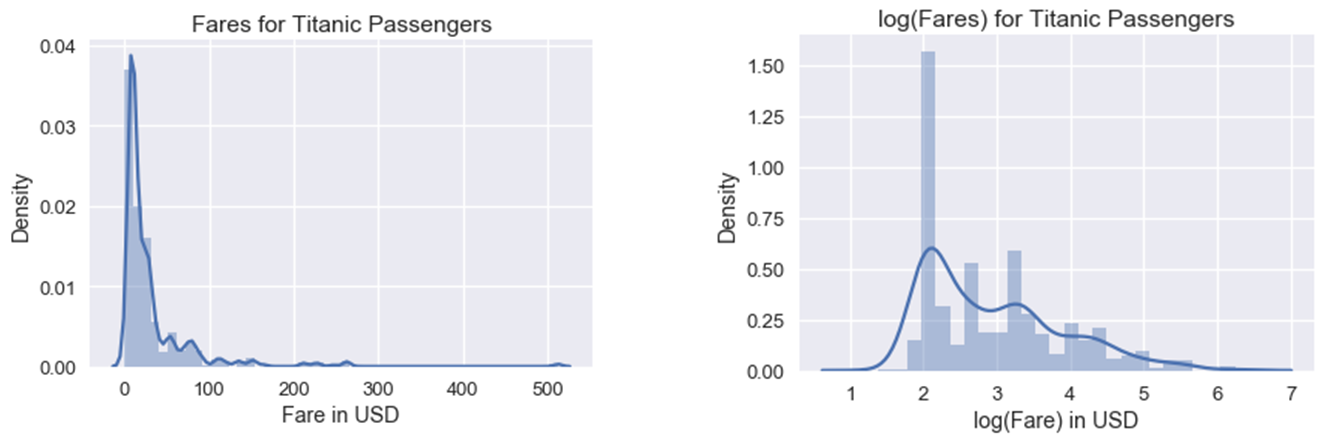
\includegraphics[scale=.43]{Bild94}
	    \end{figure}
	    When a distribution has a large dynamic range, it can be useful to take the log.
	\end{frame}
	
	
	\begin{frame}{Why straighten relationships?}
	   Now, we will look at how to linearize the scatter plot of two variables. Why?
	   \begin{itemize}
	       \item If we know what transformation made our plot of $y$ vs. $x$ linear, we can “backtrack” to figure out the exact relationship between $x$ and $y$.
	       \item Linear relationships are particularly simple to interpret.
	       \begin{itemize}
	           \item We know what slopes and intercepts mean
	       \end{itemize}
	   \end{itemize}
	        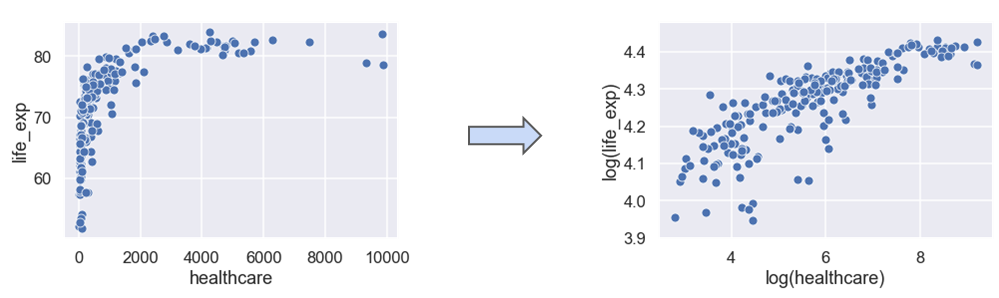
\includegraphics[scale=.43]{Bild95}
	\end{frame}
	
	
	
	\begin{frame}{Log of y-values}
	    \begin{columns}
	        \begin{column}{.5\textwidth}
	                If we take the log of our $y$-values and notice a linear relationship, we can say (roughly) that
	                \begin{equation*}
	                    \log y = ax + b
	                \end{equation*}
	                Working backwards:
	                \begin{align*}
	                    \log y &= ax + b\\
	                    y &= e^{ax+b}\\
	                    y &= e^{ax}e^b\\
	                    y &= Ce^{ax}
	                \end{align*}
	                This implies an exponential relationship in the original plot.
	        \end{column}
	        
	        
	        \begin{column}{.5\textwidth}
	                \begin{figure}
	                  % \centering
	                    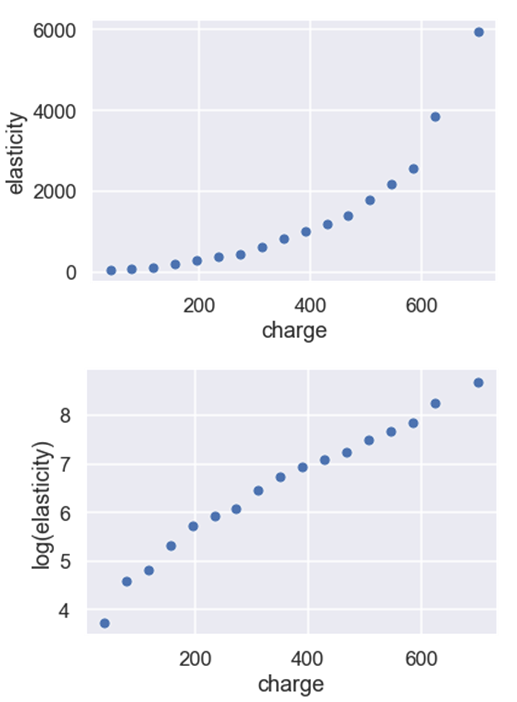
\includegraphics[scale=.3]{Bild96}
	                \end{figure}
	        \end{column}
	    \end{columns}
	\end{frame}
	
	
	\begin{frame}{Log of both x and y-values}
	    \begin{columns}
	        \begin{column}{.5\textwidth}
	                If we take the log of both axes and notice a linear relationship, we can say (roughly) that
	                \begin{equation*}
	                    \log y = a\cdot \log x + b
	                \end{equation*}
	                Working backwards:
	                \begin{align*}
	                    y &= e^{a\cdot \log x+b}\\
	                    y &= Ce^{a\cdot \log x}\\
	                    y &= Cx^a
	                \end{align*}
	                This implies a power relationship in the original plot (a one-term polynomial).
	        \end{column}
	        
	        
	        \begin{column}{.5\textwidth}
	                \begin{figure}
	                  % \centering
	                    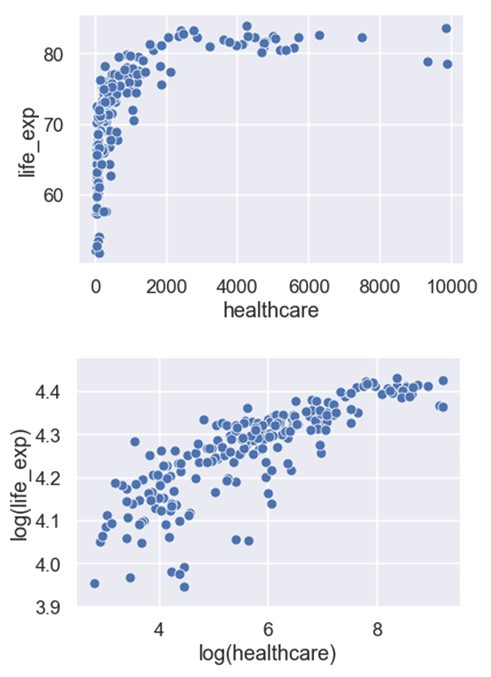
\includegraphics[scale=.33]{Bild97}
	                \end{figure}
	        \end{column}
	    \end{columns}
	\end{frame}
	
	
	
	\begin{frame}{Log transform as a “Swiss army knife”}
	    \begin{align*}
	        &y = a^k \rightarrow \log (y) = x\log (a)\\
	        &y = ax^k \rightarrow \log (y) = \log (a) + k\log (x)
	    \end{align*}
	    Properties of logarithms make them very powerful!
	\end{frame}
	
	
	
	\begin{frame}{Basic functional relations}
	    \begin{columns}
	        \begin{column}{.5\textwidth}

	               Knowing the general shapes of polynomial, exponential, and logarithmic curves\\ (regardless of base) will go a long way.
	               
	        \end{column}
	        
	        
	        \begin{column}{.5\textwidth}
	        
	                   \centering
	                   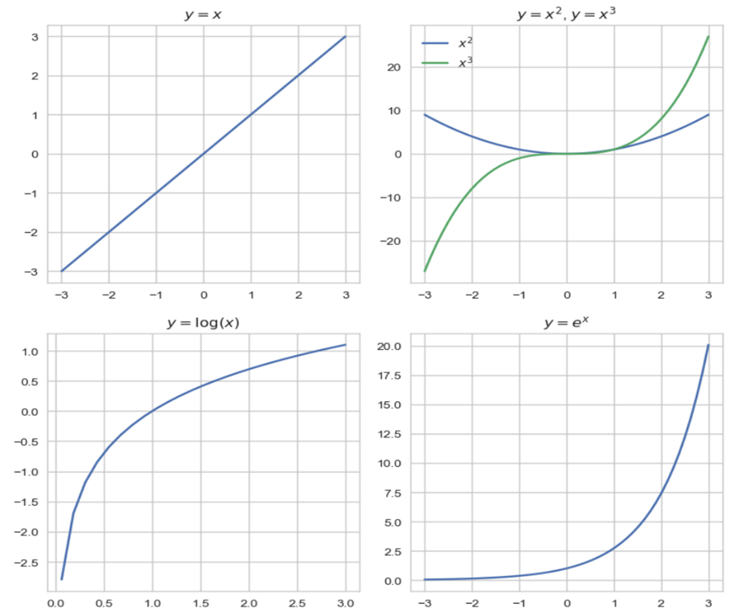
\includegraphics[scale=.35]{Bild98}

	        \end{column}
	    \end{columns}
	\end{frame}
	
	
	
% 	\begin{frame}{Tukey-Mosteller Bulge Diagram}
	
% 	    \begin{columns}
	    
% 	        \begin{column}{.5\textwidth}

% 	               This diagram can help us choose which transformation(s) to apply to our data in order to linearize it.
% 	               \begin{itemize}
% 	                   \item There are multiple solutions. Some will fit better than others.
% 	                   \item sqrt and log make a value “smaller”. Raising to a value to a power makes it “bigger”.
% 	                   \item Each of these transformations equates to increasing or decreasing the scale of an axis.
% 	               \end{itemize}
	               
% 	        \end{column}
	        
	        
% 	        \begin{column}{.5\textwidth}

% 	                   \centering
% 	                   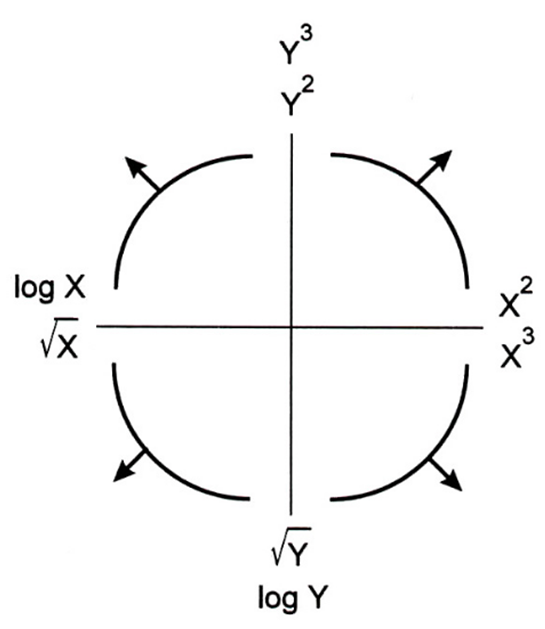
\includegraphics[scale=.35]{Bild99}

% 	        \end{column}
	        
% 	    \end{columns}
	    
% 	\end{frame}
	
	
	
	\begin{frame}{Summary}
	    \begin{itemize}
	        \item Choose appropriate scales.
	        \item Condition in order to make comparisons more natural.
	        \item Choose colors and markings that are easy to interpret correctly.
	        \item Add context and captions that help tell the story.
	        \item Smoothed estimates of distributions help with big-picture interpretation.
	        \begin{itemize}
	            \item Kernel Density Estimates are a method of smoothing data.
	        \end{itemize}
	        \item Transforming our data can linearize relationships.
	        \begin{itemize}
	            \item Helpful when we start linear modeling next lecture.
	        \end{itemize}
	        \item More generally – reveal the data!
	        \begin{itemize}
	            \item Eliminate anything unrelated to the data itself – “chart junk.”
	            \item It’s fine to plot the same thing multiple ways, if it helps fit the narrative better.
	        \end{itemize}
	    \end{itemize}
	\end{frame}
\end{document}